
\documentclass[final]{beamer}

\usepackage[scale=1.24]{beamerposter} % Use the beamerposter package for laying out the poster

\usetheme{confposter} % Use the confposter theme supplied with this template

\setbeamercolor{block title}{fg=nblue, bg=white} % Colors of the block titles
\setbeamercolor{block body}{fg=black, bg=white} % Colors of the body of blocks
\setbeamercolor{block alerted title}{fg=white, bg=dblue!70} % Colors of the highlighted block titles
\setbeamercolor{block alerted body}{fg=black, bg=dblue!10} % Colors of the body of highlighted blocks
% Many more colors are available for use in beamerthemeconfposter.sty
\setbeamercolor{itemize item}{fg=nblue, bg=white}%-----------------------------------------------------------
% Define the column widths and overall poster size
% To set effective sepwid, onecolwid and twocolwid values, first choose how many columns you want and how much separation you want between columns
% In this template, the separation width chosen is 0.024 of the paper width and a 4-column layout
% onecolwid should therefore be (1-(# of columns+1)*sepwid)/# of columns e.g. (1-(4+1)*0.024)/4 = 0.22
% Set twocolwid to be (2*onecolwid)+sepwid = 0.464
% Set threecolwid to be (3*onecolwid)+2*sepwid = 0.708

\newlength{\sepwid}
\newlength{\onecolwid}
\newlength{\twocolwid}
\newlength{\threecolwid}
\setlength{\paperwidth}{48in} % A0 width: 46.8in
\setlength{\paperheight}{36in} % A0 height: 33.1in
\setlength{\sepwid}{0.024\paperwidth} % Separation width (white space) between columns
\setlength{\onecolwid}{0.30\paperwidth} % Width of one column
\setlength{\topmargin}{-0.5in} % Reduce the top margin size
%-----------------------------------------------------------

\usepackage{graphicx}  % Required for including images

\usepackage{booktabs} % Top and bottom rules for tables


\usepackage{calrsfs}
\DeclareMathAlphabet{\pazocal}{OMS}{zplm}{m}{n}
\newcommand{\La}{\mathcal{L}}
\newcommand{\Lb}{\pazocal{L}}

\usepackage{tcolorbox}

%----------------------------------------------------------------------------------------
%	TITLE SECTION 
%----------------------------------------------------------------------------------------

\title{IMDB score prediction} % Poster title

\author{Grigor Keropyan} % Author(s)

\institute{Department of Mathematics and Mechanics at Yerevan State University} % Institution(s)

%----------------------------------------------------------------------------------------

\begin{document}

\addtobeamertemplate{block end}{}{\vspace*{2ex}} % White space under blocks
\addtobeamertemplate{block alerted end}{}{\vspace*{2ex}} % White space under highlighted (alert) blocks

\setlength{\belowcaptionskip}{2ex} % White space under figures
\setlength\belowdisplayshortskip{2ex} % White space under equations

\begin{frame}[t] % The whole poster is enclosed in one beamer frame

\begin{columns}[t] % The whole poster consists of three major columns, the second of which is split into two columns twice - the [t] option aligns each column's content to the top

\begin{column}{\sepwid}\end{column} % Empty spacer column

\begin{column}{\onecolwid} % The first column

%----------------------------------------------------------------------------------------
%	OBJECTIVES
%----------------------------------------------------------------------------------------

\begin{alertblock}{Abstract}
\begin{itemize}
\item Motivation:
Producers can use this tool to have successful films and
Customers can predict score of the film

\item Experiments:
Linear Regression, Ridge Regression, Decision Tree, Random Forest, XGBoost, 
SVM, LightGBM

\item Results:
One of the best models is Random Forest which achieved 0.44 $R^2$ score and 0.82 MSE on test set. 
Best model is LightGBM with $R^2 = 0.45$ and 0.80 MSE  on test set 

\end{itemize}
\end{alertblock}


\begin{block}{Data}
\begin{itemize}
\item Data is taken from Kaggle (Few csv files for textual data and jpg files for posters).
\item Left the movies which original language is English and have released after 1980.
\item In the dataset all NA's are dropped.
\item Total 18850 movies. For some models it is splited 70-15-15 as train-validation-test sets and for other 80-20 as train-test. For latter case cross validation is used.

\end{itemize}
\end{block}

\begin{block}{Feature Selection}

\begin{itemize}
\item Input feature categories: text (synopses), images (posters) and others (runtime, genre, director, actors)
\item For posters, using OpenCV extracted number of human faces in posters, means and standard deviations of RGB and HSB
\item For crew and cast, extracted top three actors and director
\end{itemize}

\begin{table}
  \label{dataset-table}
  \centering
  \begin{tabular}{llll}
    \toprule
    Data & Type & Dimension & Example  \\
    \midrule
    Actors & Categorical  & 1671 &  Tom Hanks   \\
    poster & Numerical & 13 & Number of faces = 0 \\
    Director & Categorical & 491 & Howard Deutch \\
    Runtime & Numerical & 1 & 121 (minutes) \\
    Genre & Categorical & 23 & Documentation \\
    Synopses & Categorical & 3712 & Once \\
    \bottomrule
  \end{tabular}
\end{table}

\end{block}

\end{column} % End of the first column

\begin{column}{\sepwid}\end{column} % Empty spacer column

\begin{column}{\onecolwid} % Begin a column which is two columns wide (column 2)
\begin{block}{Models}
\begin{itemize}
\item Linear Regression: $\theta^* = argmin_\theta$ $\frac{1}{n} \Sigma_{i=1}^{n}
(\theta^Tx^{(i)} - y^{(i)})^2$

\item Linear Regression: $\theta^* = argmin_\theta$ $\frac{1}{n} \Sigma_{i=1}^{n}
(\theta^Tx^{(i)} - y^{(i)})^2 + \lambda||\theta||^2$

\item XGBoost: $\Lb (\phi) = \Sigma_i l(\hat{y}_i, y_i) + \Sigma_k \Omega (f_k) $, where  $\Omega (f) = \gamma T + \frac{1}{2}\lambda ||\omega||^2 $

\item Decision Trees and Random Forest: A random forest is a meta estimator that fits a number of classifying decision trees on various sub-samples of the dataset and uses averaging to improve the predictive accuracy and control over-fitting.

\item LightGBM: our best model: \\
LightGBM is a gradient boosting framework that uses tree based learning algorithms. It is designed to be distributed and efficient and have a few advantages.


\begin{minipage}{0.3\textwidth}
\begin{figure}[H]
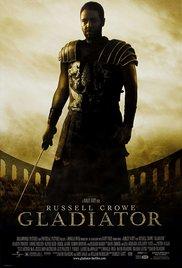
\includegraphics[width=0.9\textwidth]{172495.jpg}
\end{figure}

\end{minipage} \hfill
\begin{minipage}{0.3\textwidth}
\begin{tcolorbox}
A former Roman General sets out to exact vengeance against the corrupt emperor who murdered his family and sent him into slavery.
\end{tcolorbox}
\end{minipage} \hfill
\begin{minipage}{0.3\textwidth}
\begin{tcolorbox}
\begin{itemize}
\item Director: Ridley Scott
\item Actors:  Russell Crowe, Joaquin Phoenix, Connie Nielsen
\item Genre:  Action, Adventure, Drama 
\item Runtime: 155 min
\end{itemize}
\end{tcolorbox}
\end{minipage} \hfill

\begin{tcolorbox}
\centering
LightGBM
\end{tcolorbox}

\end{itemize}
\end{block}

\begin{block}{Results}

\begin{table}
  \centering
  \begin{tabular}{lllll}
    \toprule
    Method & Train MSE & Test MSE & Train $R^2$ & Test $R^2$  \\
    \midrule
    Linear Regression & 0.4366 & 1.3918 & 0.7043 & 0.0668   \\
    Ridge Regression & 0.5333 & 0.9824 & 0.6389 & 0.3413   \\
    Decision Tree & 0.8440 & 0.9153 & 0.4285 & 0.3863   \\
    Random Forest & 0.8277 & 0.8290 & 0.2543 & 0.4441   \\
    XGBoost & 0.5160 & 0.8375 & 0.6506 & 0.4384 \\
    SVR & 0.5735 & 0.9294 & 0.6117 & 0.3768 \\
    LightGBM & 0.6488 & 0.8067 & 0.5592 & 0.4513 \\
        \bottomrule
  \end{tabular}
\end{table}

\end{block}

\begin{itemize}
\item The first six models were trained on 13194 training samples, while hyperparameters were selected using 2828 validation samples and evaluated on 2828 test samples. However, in the case of LightGBM dataset is splited into train and test set with 15080, 3770 samples in each.
\item LightGBM is the best model among all of the models.

\end{itemize}

\end{column} % End of the second column

\begin{column}{\sepwid}\end{column} % Empty spacer column

\begin{column}{\onecolwid} % The third column

%\setbeamercolor{block title}{fg=red,bg=white}
\begin{block}{Comparison with previous work}
In the Table 1 the model is compared with the Stanford students paper [1].
In this models out Random Forest achieved better accuracy in the sense of MSE and $R^2$ compared with [1]. Moreover, the LIghtGBM model achieved 0.8 MSE and 0.45 $R^2$ which is better than our Random Forest model.

\begin{table}
  \caption{Comparison with [1]}
  \label{cmp_results-table}
  \centering
  \begin{tabular}{lllll}
    \toprule
    Method & our MSE & [1] MSE &  our $R^2$  & [1] $R^2$  \\
    \midrule
    Linear Regression & 1.3918 & 0.9302  & 0.0668  & 0.3745   \\
    Ridge Regression & 0.9824 & 0.8775  & 0.3413 & 0.4099  \\
    Decision Tree & 0.9153  & 0.8959 & 0.3863  & 0.3975 \\
    Random Forest & 0.8290  & 0.8546 & 0.4441 & 0.4253 \\
    SVR & 0.9294 & 0.8765 & 0.3768  & 0.4109 \\
        \bottomrule
  \end{tabular}
  
\end{table}
\end{block}

\begin{block}{Feature Importance}
Feature importance in the Random Forest model is shown in the following figure. From the bar plot we can conclude that runtime and specific genre is important for the IMDB score.

\begin{figure}
	\centering
	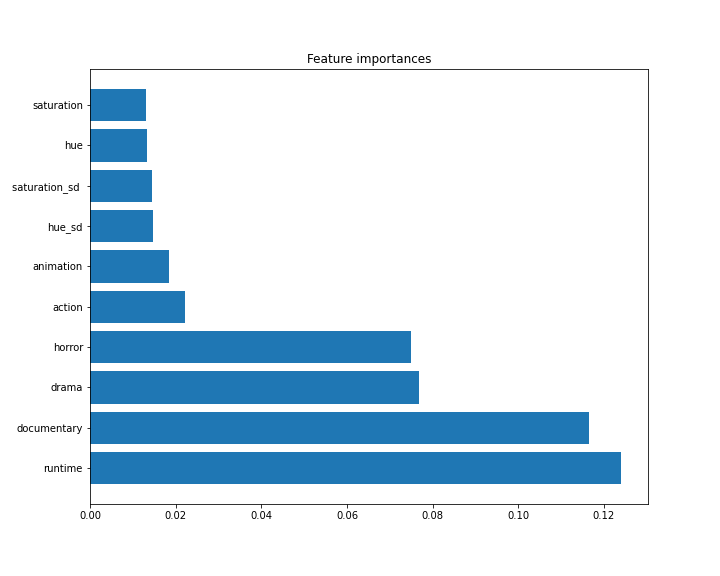
\includegraphics[width=1.2\linewidth, height=0.35\textheight, keepaspectratio]{../plots/feature_importancvce.png}
	\label{fig:feature_imp}
\end{figure}
\end{block}

\begin{block}{References}
\small
[1] Yichen Yang et al., {\it "Predicting Movie Ratings with Multimodal Data"},
\url{http://cs229.stanford.edu/proj2019aut/data/assignment_308832_raw/26260680.pdf}.
\end{block}

\end{column} % End of the third column

\end{columns} % End of all the columns in the poster

\end{frame} % End of the enclosing frame

\end{document}
